%%%%%%%%%%%%%%%%%%%%%%%%%%%%%%%%%%%%%%%%%%%%%%%%%%%%%%%%%%%%%%%%%%%%%%
% Câu chưa có mã dạng — cần gắn %[..] rồi chuyển vào đúng file dạng
% Số câu: 1  (sinh tự động bởi tach_cau.py; từ nay thầy sửa trực tiếp file này)
%%%%%%%%%%%%%%%%%%%%%%%%%%%%%%%%%%%%%%%%%%%%%%%%%%%%%%%%%%%%%%%%%%%%%%

%%%%%%%%%%%%%%%% ĐÚNG/SAI %%%%%%%%%%%%%%%%

% nguồn: Phan1_Lop_12_Dai_so_Chuong_1
\begin{ex}%[ma:4e74e127]
	2%[2D1H3-1] 
	Cho hàm số $y=f(x)$ liên tục trên ${\bf \mathbb{R}}$ và có bảng biến thiên  trong hình vẽ dưới đây:
	\begin{center}
		\begin{tikzpicture}
			\tkzTabInit 
				[lgt=1.5,espcl=2] 
				 {$x$/1.2,$f’(x)$/1,$f (x)$/2}
				 {$-\infty$,$-1$,$0$,$1$,$+\infty$}
			 \tkzTabLine{,-,0,+,0,-,0,+,}
			\tkzTabVar{+/ $+\infty$,-/ $-2 $,+/$-1$,-/ $-2  $,+/ $+\infty$}
		\end{tikzpicture}
	\end{center}
	\choiceTF 
		{Hàm số đồng biến trên mỗi khoảng $\left(-1; 0\right)$; $\left(1;+\infty \right)$ và nghịch biến trên  khoảng $\left(-\infty; 1\right)$}
		{\True Hàm số đạt cực tiểu tại $x=\pm 1$ và có giá trị cực tiểu là  $y=-2$}
		{Hàm số đạt giá  trị lớn nhất tại $x=0$}
		{\True Tổng giá trị lớn nhất  và giá trị nhỏ nhất của hàm số trên đoạn $\left[-1; 1\right]$ bằng $-3$}
	 \loigiai{
		\begin{itemchoice}
			\itemch Hàm số đồng biến trên  mỗi khoảng $\left(-1; 0\right)$; $\left(1;+\infty \right)$ và nghịch biến trên khoảng $\left(-\infty;-1\right)$.
			\itemch Hàm số đạt cực tiểu  tại $x=\pm 1$ và có giá trị cực tiểu là $y=-2$.
			\itemch  Hàm số đạt không có giá trị lớn nhất.
			\itemch $M=\displaystyle \max_{[-1;1]} f(x)= -1$ và $ m =\displaystyle \min_{[-1;1]} f(x)=-2  $ nên $M+m =-3$.
		\end{itemchoice}
	 }
\end{ex}
